\chapter{Credit Risk}

\section{Credit Risk management}
Part of the daily business of a financial institution is the credit risk assessment of existing and new customers. The result is used to decide if they want to decline or grant a credit application and, among other things, to set the required regulatory capital. Credit risk assessment is performed during the whole lifetime of an exposure. It starts with the approval of a transaction and is continuously monitored afterward. Corporate clients usually need to submit financial reports regularly, which are then analyzed by their bank advisor and credit analyst, while it is done automatically for retail customers via behavior scoring. The information used during the application scoring is limited because the applicant mainly provides it at the start of a new contract. It generally covers variables about their financial health, e.g., income and outstanding debt. For the behavior scoring model, internal historical data is used, for example, the borrower's payment history and credit utilization. The behavior model generally shows a better predictive performance than the application model. If a decline in financial health or behavior rating is detected, the bank may try to decrease the overdraft limit to regulate the credit risk. In the case of delayed payments, the early collection process starts, where affected customers are contacted and an alternative payment plan will be negotiated. If all interventions fail, defaulted exposures may be sold or outsourced to collection companies for further processing, like the sale of collateral. \cite[p.~7]{Witzany:2017}

\section{Default Rate and Probability of Default}
\label{sec:dr_pd}
A critical risk measure is the probability of default (PD), which is an estimate of the likelihood of a borrower failing to pay back their financial obligations in a given time period. Depending on the analyzed portfolio, the expected number of defaults can vary. In the corporate segment, individual defaults might already be seen as an indicator of a bank's failing credit assessment process and decision. In contrast, a higher number of defaults can be expected in the retail sector. On the contrary, profit is generated if the income gained from non-defaulted customers covers the loss from the defaulted portion of the portfolio. \cite[p.~2]{Witzany:2017}

\medskip
In the Capital Requirements Regulation (Capital Requirements Regulation, Article 178(1)), the definition of default is stated as:

\begin{quote}

A default shall be considered to have occurred with regard to a particular obligor when either or both of the following have taken place:
\begin{itemize}
\item[(a)] the institution considers that the obligor is unlikely to pay its credit obligations to the institution, the parent undertaking or any of its subsidiaries in full, without recourse by the institution to actions such as realising security;
\item[(b)] the obligor is more than 90 days past due on any material credit obligation to the institution, the parent undertaking or any of its subsidiaries. Competent authorities may replace the 90 days with 180 days for exposures secured by residential property or SME commercial immovable property in the retail exposure class, as well as exposures to public sector entities. The 180 days shall not apply for the purposes of point (m) Article 36(1) or Article 127.

\end{itemize}

In the case of retail exposures, institutions may apply the definition of default laid down in points (a) and (b) of the first subparagraph at the level of an individual credit facility rather than in relation to the total obligations of a borrower.

\end{quote}

A time period has to be defined in which a default event is observed. A common observation window is one year; an illustration is visible in Figure \ref{fig:cr_timeperiod}. The default rate per category (e.g., month, rating grade) is then calculated as the number of defaults divided by the total number of customers (Eq. \ref{eq:cr_dr}). \cite[pp.~20-21]{Witzany:2017}

\begin{equation}
DR_{i} = \frac{d_{i}}{n_{i}} \label{eq:cr_dr}
\end{equation}
where:
\begin{conditions}
 d_{i}  & number of defaults in class i \\
 n_{i}  & number of observations in class i
\end{conditions}

\begin{figure}[H]
	\centering
	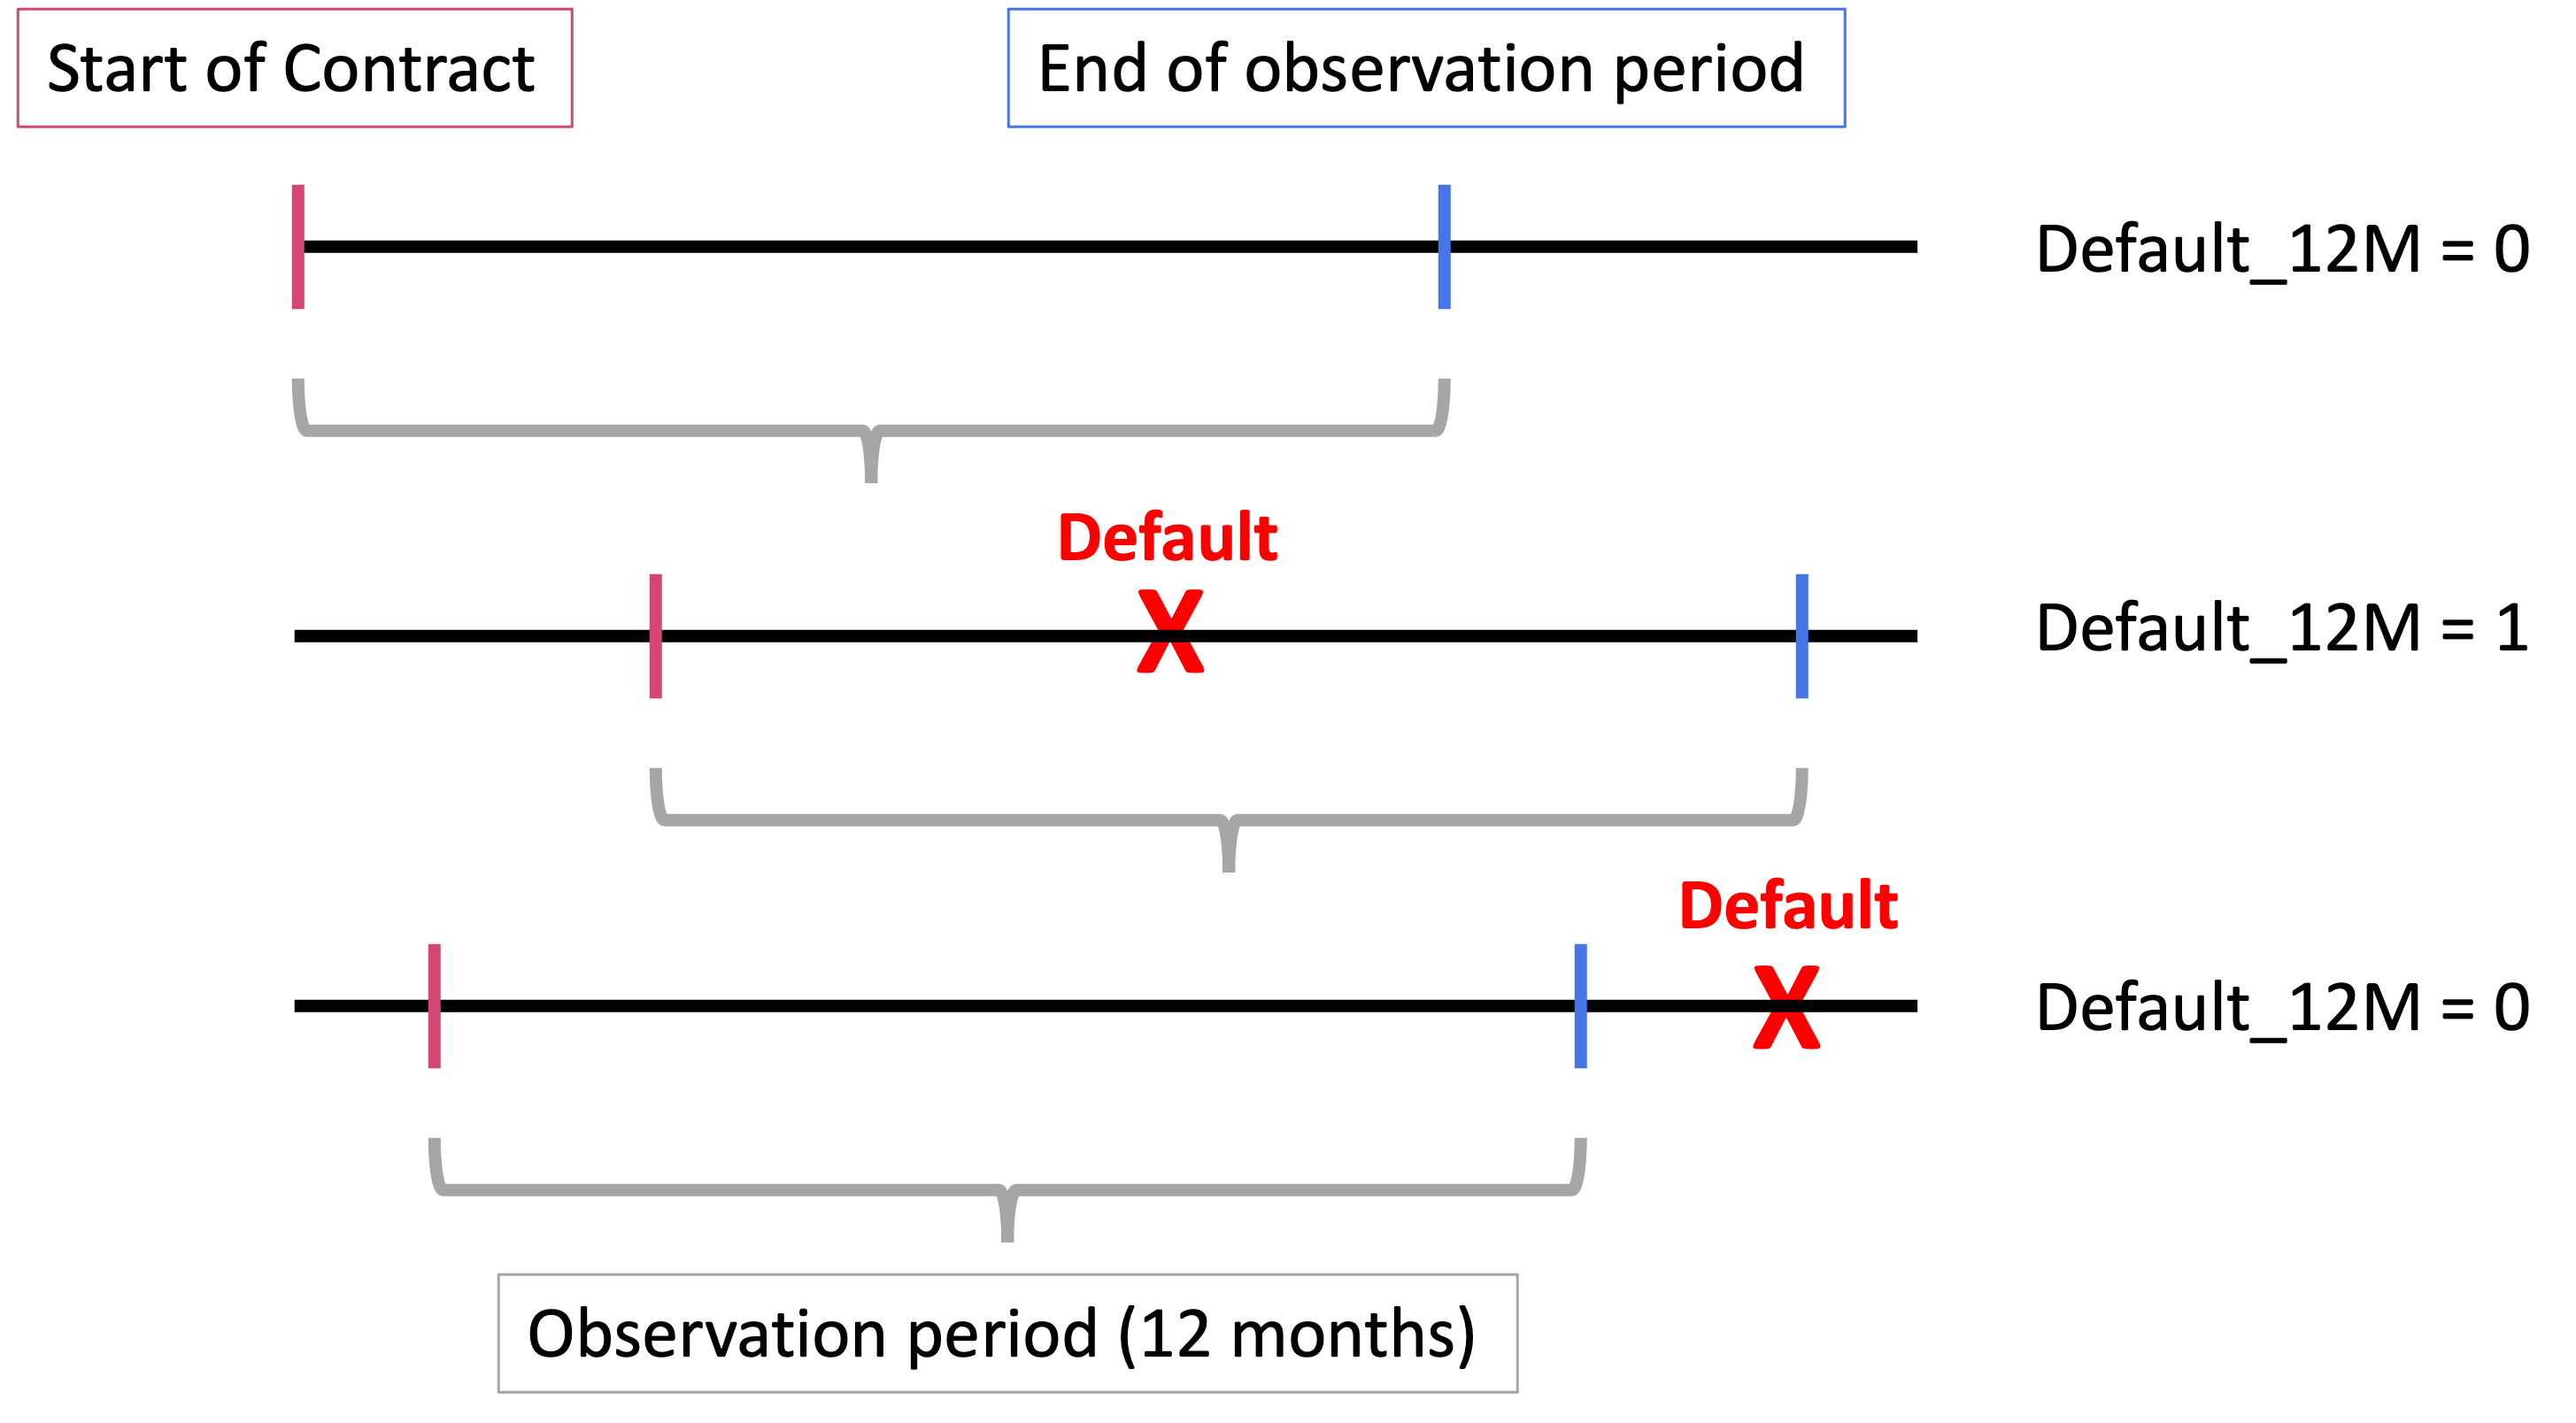
\includegraphics[width=.625\textwidth]{./CR__ObservationPeriod.png}
    \caption{Observation period after reference point}
    \label{fig:cr_timeperiod}
\end{figure}

\section{Regulatory Framework}

\subsection{History of Regulatory Framework}

The Basel Committee on Banking Supervision sets the regulatory framework, which consists of all regulators of the most developed countries. The goal is to define a high standard for risk management and internal controls and establish a risk-sensitive calculation process of the regulatory capital for banks worldwide. The First Capital Accord was published in 1988 and has been adapted and reformed numerous times. The New Capital Accord, also known as Basel II, was first issued in 2004 and underwent multiple amendments, especially after the financial crisis until July 2009. The European Union motivated the integration of these regulations by the Implementation Directive CAD 2006. At the end of 2010, a new reform called Basel III was approved. \cite[p.~13]{Witzany:2017}

\subsection{Credit Risk Regulatory Capital}

The credit risk capital requirement calculation was significantly improved compared to the First Capital Accord. The total loss of a bank is split into expected and unexpected loss (Figure \ref{fig:cr_elul}). The former should be covered by revenue; for the latter, a bank must allocate an appropriate level of capital. In the original approach, each exposure was assigned to one of four risk categories and then a multiplier ranging from 0-100\% was applied. Regulations now allow the Standardized (SA), Foundation or Advanced Internal Rating Based (IRB-F, IRB-A) Approach. The Standard Approach defines five risk buckets for calculating regulatory capital, and it also allows the use of external ratings. For the IRB approach, internal models estimate input parameters of the regulatory formulas, which then result in risk weights for each exposure used in the calculation of the regulatory capital. The formulas are given in Eq. \ref{eq:PD_cap1}-\ref{eq:PD_cap4}. The IRB-F approach only permits the estimation of the PD. In contrast, for the IRB-A approach, the risk parameters Loss Given Default, Exposure at Default, Conversion Factor and Effective Maturity are additionally derived from internal models. While the corporate segment allows for both IRB-F and IRB-A approaches, the retail portfolio is limited to the IRB-A approach. \cite[15-17]{Witzany:2017} \cite[p.~59]{BCBS:2004}


\begin{figure}[H]
	\centering
	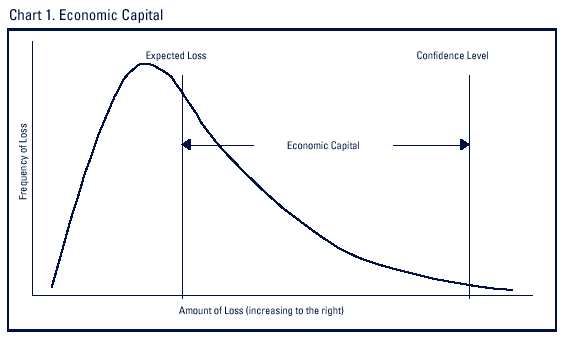
\includegraphics[width=.625\textwidth]{./CR__EL_UL_capital.png}
    \caption{Economical Capital, Expected and Unexpected Losses, Source: \cite{FDIC:2023}}
    \label{fig:cr_elul}
\end{figure}

\begin{align} 
\rho &= \rho_{min} \times \frac{1 - e^{-k \times PD}}{1 - e^{-k}} +  \rho_{max} \times \left((1 - \frac{1 - e^{-k \times PD}}{1 - e^{- k}}\right) \label{eq:PD_cap1}\\[15pt]
\text{b} &= (0.11852 - 0.05478 \times ln(PD))^2 \\[15pt]
\text{MA} &= \frac{1 + (Maturity - 2.5) \times b}{1 - 1.5 \times b} \\[15pt]
\text{K} &= \left(\Phi \left[\frac{\Phi^{-1}(PD) + \sqrt{\rho} \times \Phi^{-1}(0.999)}{\sqrt{1 - \rho}}\right] - PD\right) \times LGD \times MA \label{eq:PD_cap4}
\end{align}
where:
\begin{conditions}
\rho 					& Correlation \\
\rho_{min}, \rho_{max}  & minimum and maximum correlation per class \\
k  						& rise coefficient per class \\
b 						& Maturity adjustment \\
MA						& Residual Maturity Adjustment Factor \\
K						& Capital requirement
\end{conditions}

\subsection{Challenges and Limitations}
Good data is of utmost importance for the credit risk assessment. While it will be used for modeling purposes, it is also essential that already-known negative information about customers is available and considered. Examples include internal information, such as a client with a history of fraudulent activity during a credit application or credit bureau data, where negative credit information is made available for all participants. Institutions in Austria providing these kinds of information are Kreditschutzverband (KSV) and CRIF.

Other possible challenges are the constant change in economic conditions and regulatory frameworks, which influence the PD estimates. In addition, during the PD estimation process, the default events of individual borrowers are assumed to be independent, which does not adequately capture behavioral risks (e.g., strategic default) or systemic risks (e.g., market-wide shocks) that can affect multiple borrowers simultaneously. Therefore, PD models must be continuously refined and adapted to accurately reflect the current economic situation. \cite[p.~8]{Witzany:2017}